
% TODO: \usepackage{graphicx} required
\begin{figure}[H]
	\centering
	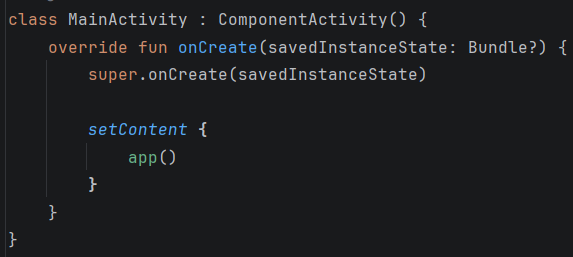
\includegraphics[width=0.85\textwidth]{Practica1_codigo1}
	\caption{Estructura inicial de MainActivity.}
	\label{fig:practica1codigo1}
\end{figure}

\begin{figure}[H]
	\centering
	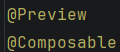
\includegraphics[width=0.85\textwidth]{Practica1_codigo2}
	\caption{Definición de la función composable y habilitación de la vista previa mediante @Preview.}
	\label{fig:practica1codigo2}
\end{figure}

\begin{figure}[H]
	\centering
	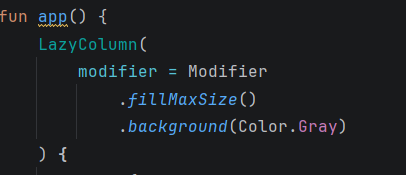
\includegraphics[width=0.85\textwidth]{Practica1_codigo3}
	\caption{Implementación de LazyColumn para organizar los elementos de la interfaz en una lista vertical desplazable.}
	\label{fig:practica1codigo3}
\end{figure}

\begin{figure}[H]
	\centering
	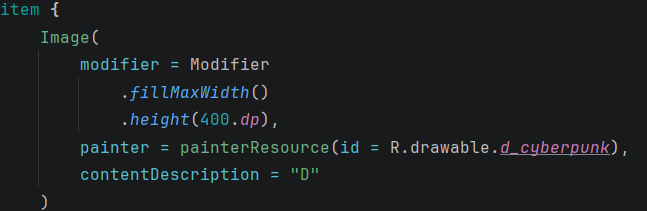
\includegraphics[width=0.85\textwidth]{Practica1_codigo4}
	\caption{Configuración del componente Image para mostrar una imagen y establecer sus dimensiones.}
	\label{fig:practica1codigo4}
\end{figure}

\begin{figure}[H]
	\centering
	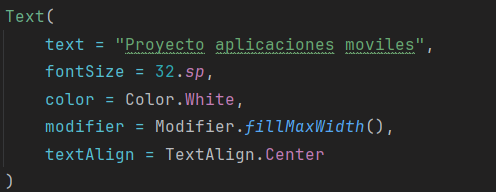
\includegraphics[width=0.85\textwidth]{Practica1_codigo5}
	\caption{Configuración del componente Text para mostrar un mensaje con tamaño, color y alineación personalizados.}
	\label{fig:practica1codigo5}
\end{figure}

\begin{figure}[H]
	\centering
	
\includegraphics[width=0.45\textwidth]{Practica1_codigo6}
	\caption{Resultado de la implementación de los componentes Image y Text en el emulador de Android.}
	\label{fig:practica1codigo6}
\end{figure}

\begin{figure}[H]
	\centering
	
\includegraphics[width=0.45\textwidth]{Practica1_codigo7}
	\caption{Ejecución de la interfaz de usuario en el emulador de Android con formato de dispositivo móvil.}
	\label{fig:practica1codigo7}
\end{figure}

\begin{figure}[H]
	\centering
	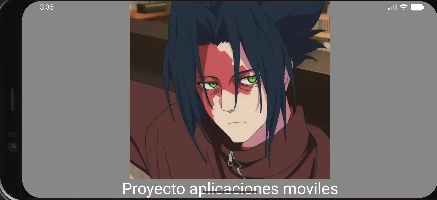
\includegraphics[width=0.85\textwidth]{Practica1_codigo8}
	\caption{Visualización de la interfaz en orientación horizontal, demostrando su adaptación al cambio de orientación del dispositivo móvil.}
	\label{fig:practica1codigo8}
\end{figure}

\begin{figure}[H]
	\centering
	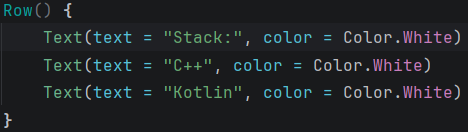
\includegraphics[width=0.85\textwidth]{Practica2_codigo1}
	\caption{Implementación del componente Row para organizar elementos de texto de manera horizontal.}
	\label{fig:practica2codigo1}
\end{figure}

\begin{figure}[H]
	\centering
	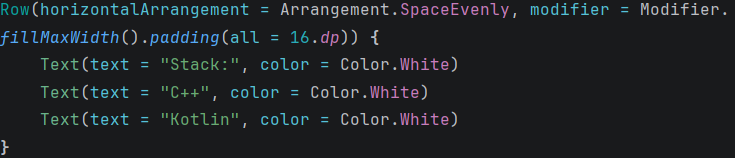
\includegraphics[width=0.85\textwidth]{Practica2_codigo2}
	\caption{Configuración de Row mediante Arrangement.SpaceEvenly y Modifier para distribuir los elementos horizontalmente.}
	\label{fig:practica2codigo2}
\end{figure}

\begin{figure}[[H]
	\centering
	
\includegraphics[width=0.45\textwidth]{Practica2_codigo3}
	\caption{Visualización de LazyRow con elementos distribuidos horizontalmente en orientación vertical}
	\label{fig:practica2codigo3}
\end{figure}


\begin{figure}[H]
	\centering
	
\includegraphics[width=0.85\textwidth]{Practica2_codigo4}
	\caption{Adaptación de la interfaz y visualización de LazyRow en orientación horizontal}
	\label{fig:practica2codigo5}
\end{figure}


\begin{figure}[H]
	\centering
	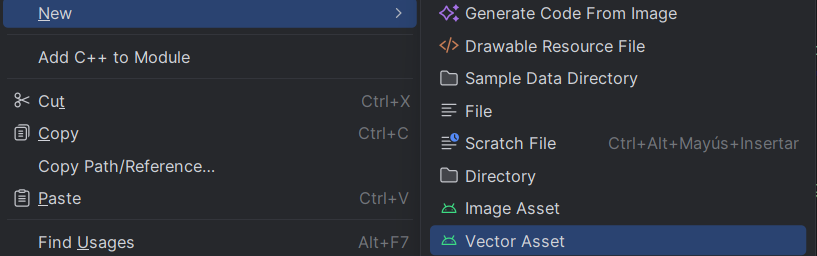
\includegraphics[width=0.85\textwidth]{Practica3_codigo1}
	\caption{Creación de un nuevo asset en la carpeta drawable}
	\label{fig:practica3codigo1}
\end{figure}

\begin{figure}[H]
	\centering
	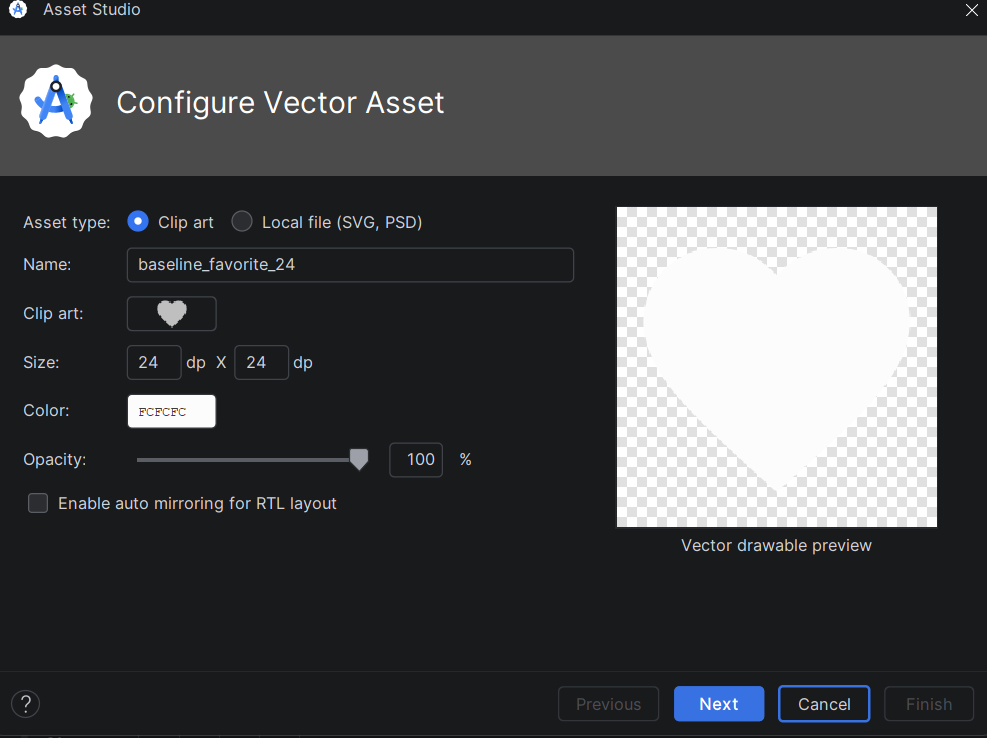
\includegraphics[width=0.85\textwidth]{Practica3_codigo2}
	\caption{Creación del nuevo asset favorite1}
	\label{fig:practica3codigo2}
\end{figure}

\begin{figure}[H]
	\centering
	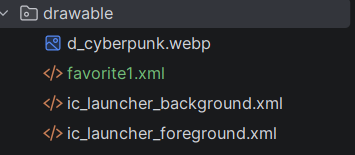
\includegraphics[width=0.85\textwidth]{Practica3_codigo3}
	\caption{Vertical asset en la carpeta drawable}
	\label{fig:practica3codigo3}
\end{figure}

\begin{figure}[H]
	\centering
	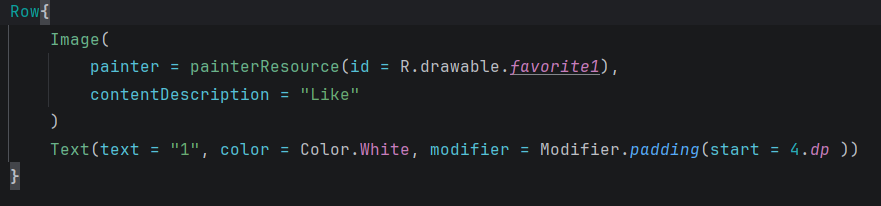
\includegraphics[width=0.85\textwidth]{Practica3_codigo4}
	\caption{Vertical asset en la carpeta drawable}
	\label{fig:practica3codigo4}
\end{figure}


\begin{figure}[H]
	\centering
	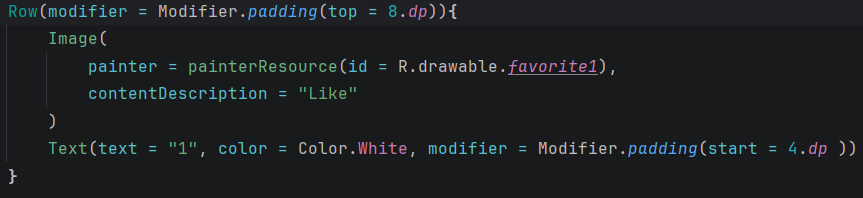
\includegraphics[width=0.85\textwidth]{Practica3_codigo5}
	\caption{Vertical asset en la carpeta drawable}
	\label{fig:practica3codigo5}
\end{figure}

\begin{figure}[H]
	\centering
	
\includegraphics[width=0.45\textwidth]{Practica3_codigo6}
	\caption{Verificacion de la creación del asset favorite1}
	\label{fig:practica3codigo6}
\end{figure}